\documentclass[10pt,letterpaper]{article}
\usepackage[utf8]{inputenc}
\title{EV 2.8 CALCULAR LOS COMPONENTES DE CIRCUITOS DE ACTIVACION DE TRANSISTORES DE POTECIA}
\author{Ascencio De Leon Agustin}
\usepackage[spanish]{babel}
\usepackage{graphicx}
\graphicspath{{imagenes/}}
\usepackage[left=2.5cm,top=2.5cm,bottom=3cm,right=2.5cm]{geometry}


\begin{document}
\maketitle
\begin{figure}[h!]
\centering 
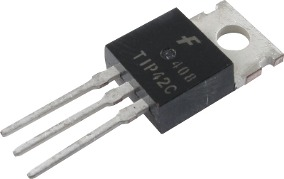
\includegraphics[scale=1]{1}
\end{figure}
\newpage
\section{Transistores de potencia}
El funcionamiento y utilización de los transistores de potencia es idéntico al de los transistores normales, teniendo como características especiales las altas tensiones e intensidades que tienen que soportar y, por tanto, las altas potencias a disipar.

Existen tres tipos de transistores de potencia:

1. bipolar.\\
2. unipolar o FET (Transistor de Efecto de Campo).\\
3. IGBT.\\
El IGBT ofrece a los usuarios las ventajas de entrada MOS, más la capacidad de carga en corriente de los transistores bipolares:

1. Trabaja con tensión.\\
2. Tiempos de conmutación bajos.\\
3. Disipación mucho mayor (como los bipolares).\\
Nos interesa que el transistor se parezca, lo más posible, a un elemento ideal:

1. Pequeñas fugas.\\
2.Alta potencia.\\
Bajos tiempos de respuesta (ton , toff), para conseguir una alta frecuencia de funcionamiento.
Alta concentración de intensidad por unidad de superficie del semiconductor.
Que el efecto avalancha se produzca a un valor elevado ( VCE máxima elevada).
Que no se produzcan puntos calientes (grandes di/dt ).
Una limitación importante de todos los dispositivos de potencia y concretamente de los transistores bipolares, es que el paso de bloqueo a conducción y viceversa no se hace instantáneamente, sino que siempre hay un retardo (ton , toff). Las causas fundamentales de estos retardos son las capacidades asociadas a las uniones colector - base y base - emisor y los tiempos de difusión y recombinación de los portadores.


\section{Principios básicos de funcionamiento}
La diferencia entre un transistor bipolar y un transistor unipolar o FET es el modo de actuación sobre el terminal de control. En el transistor bipolar hay que inyectar una corriente de base para regular la corriente de colector, mientras que en el FET el control se hace mediante la aplicación de una tensión entre puerta y fuente. Esta diferencia vienen determinada por la estructura interna de ambos dispositivos, que son substancialmente distintas.

Es una característica común, sin embargo, el hecho de que la potencia que consume el terminal de control (base o puerta) es siempre más pequeña que la potencia manejada en los otros dos terminales.

En resumen, destacamos tres cosas fundamentales:

En un transistor bipolar IB controla la magnitud de IC.\\
En un FET, la tensión VGS controla la corriente ID.\\
En ambos casos, con una potencia pequeña puede controlarse otra bastante mayor.\\
\newpage
\section{Tiempos de conmutación}
\begin{figure}[h!]
\centering 
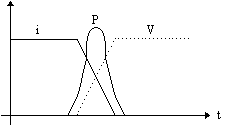
\includegraphics[scale=1]{3}
\end{figure}
Cuando el transistor está en saturación o en corte las pérdidas son despreciables. Pero si tenemos en cuenta los efectos de retardo de conmutación, al cambiar de un estado a otro se produce un pico de potencia disipada, ya que en esos instantes el producto IC x VCE va a tener un valor apreciable, por lo que la potencia media de pérdidas en el transistor va a ser mayor. Estas pérdidas aumentan con la frecuencia de trabajo, debido a que al aumentar ésta, también lo hace el número de veces que se produce el paso de un estado a otro.
Podremos distinguir entre tiempo de excitación o encendido (ton) y tiempo de apagado (toff). A su vez, cada uno de estos tiempos se puede dividir en otros dos.
\begin{figure}[h!]
\centering 
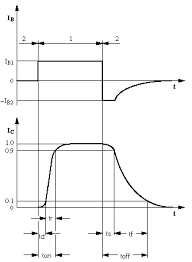
\includegraphics[scale=1]{2}
\end{figure}
\newpage
Tiempo de retardo (Delay Time, td): Es el tiempo que transcurre desde el instante en que se aplica la señal de entrada en el dispositivo conmutador, hasta que la señal de salida alcanza el 10% de su valor final.

Tiempo de subida (Rise time, tr): Tiempo que emplea la señal de salida en evolucionar entre el 10% y el 90% de su valor final.

Tiempo de almacenamiento (Storage time, ts): Tiempo que transcurre desde que se quita la excitación de entrada y el instante en que la señal de salida baja al 90% de su valor final.

Tiempo de caída (Fall time, tf): Tiempo que emplea la señal de salida en evolucionar entre el 90% y el 10% de su valor final.

Por tanto, se pueden definir las siguientes relaciones :
\begin{figure}[h!]
\centering 
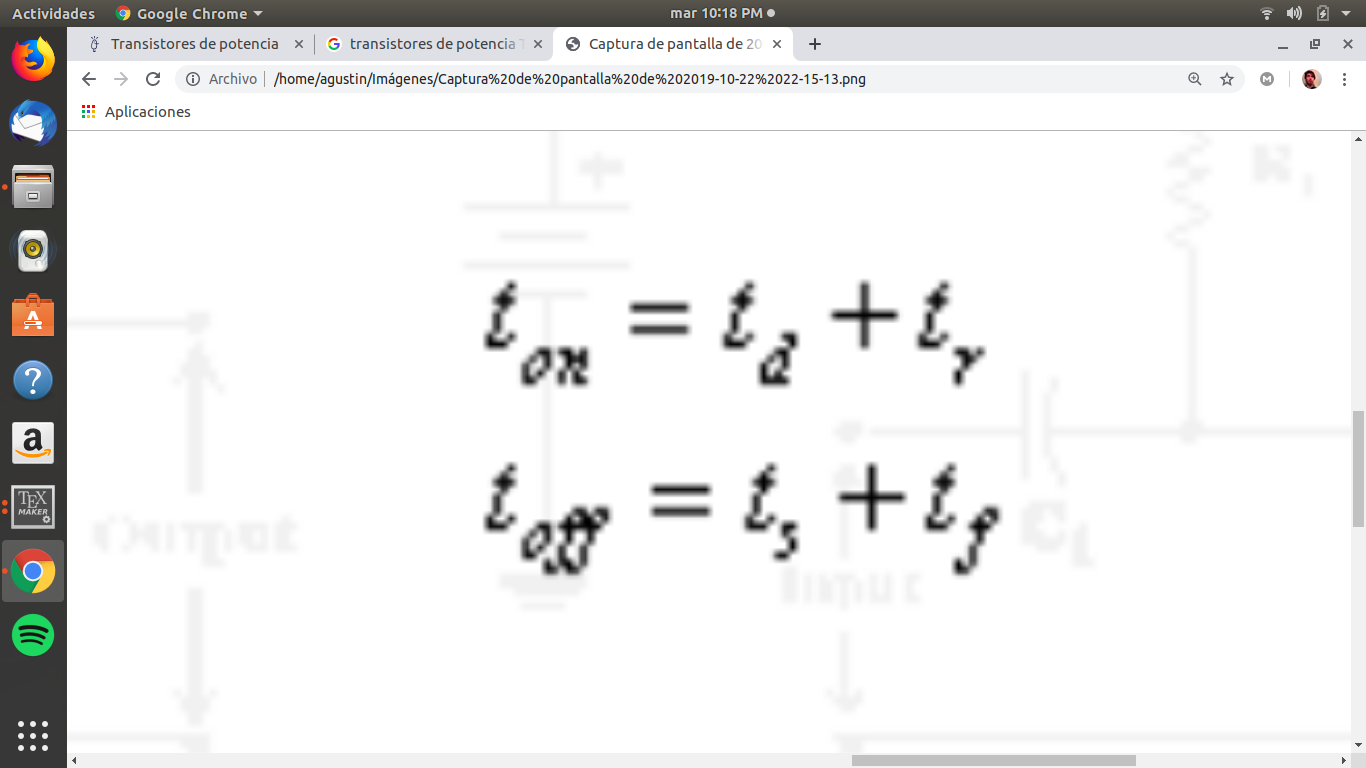
\includegraphics[scale=.1]{5}
\end{figure}
\section{Otros parámetros importantes}
\begin{figure}[h!]
\centering
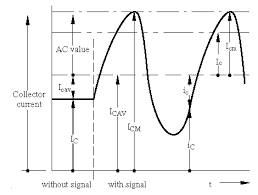
\includegraphics[scale=1]{4}
\end{figure}

Corriente media: es el valor medio de la corriente que puede circular por un terminal (ej. ICAV, corriente media por el colector).
Corriente máxima: es la máxima corriente admisible de colector (ICM) o de drenador (IDM). Con este valor se determina la máxima disipación de potencia del dispositivo.

VCBO: tensión entre los terminales colector y base cuando el emisor está en circuito abierto.
VEBO: tensión entre los terminales emisor y base con el colector en circuito abierto.

Tensión máxima: es la máxima tensión aplicable entre dos terminales del dispositivo (colector y emisor con la base abierta en los bipolares, drenador y fuente en los FET).

Estado de saturación: queda determinado por una caída de tensión prácticamente constante. VCEsat entre colector y emisor en el bipolar y resistencia de conducción RDSon en el FET. Este valor, junto con el de corriente máxima, determina la potencia máxima de disipación en saturación.

Relación corriente de salida - control de entrada: hFE para el transistor bipolar 

\end{document}